\chapter{Estrutura do código fonte do Gerador de Consultas SQL para PostGIS (PostNET)}

A ferramenta de geração de consultas em SQL para PostGIS serve como uma interface gráfica para estimular o aprendizado e a utilização da ferramenta PostGIS assim como uma ferramenta para o ensino da linguagem SQL. Além disso, o módulo se propõe a servir como uma plataforma de ensino da manipulação e análise de dados espaciais utilizando banco de dados geográficos. O software foi desenvolvido no Microsoft Visual Studio 2015 utilizando a linguagem de programação C\#. O código a seguir é referente ao módulo PostGIS que pode ser visualizado na Figura \ref{fig:postnetguiquery}:

	\begin{figure}
		\centering
		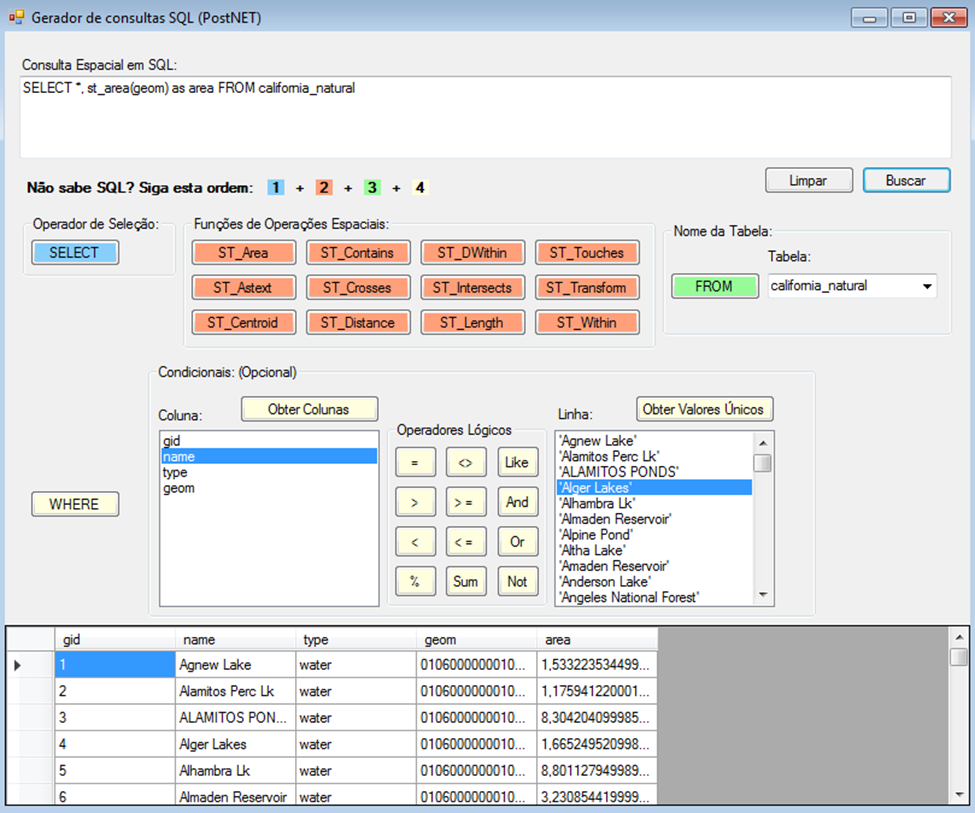
\includegraphics[width=1\linewidth]{data/postnet_gui_query}
		\caption{Interface gráfica do Gerador de Consultas SQL (PostGIS)}
		\label{fig:postnetguiquery}
	\end{figure}

\newpage
	
\begin{lstlisting}
	using System;
	using System.Collections.Generic;
	using System.ComponentModel;
	using System.Data;
	using System.Drawing;
	using System.Linq;
	using System.Text;
	using System.Windows.Forms;
	using Npgsql;
	
	namespace espacoGIS
	{
	public partial class sqlQuery : Form
	{
	public string sql;
	
	// mFrom = false => uma tabela (1x geom)
	// mFrom = true => duas tabelas (2x geom)
	bool mFrom = false;
	
	public sqlQuery()
	{
	InitializeComponent();
	getTables();
	}
	
	/// <summary>
	/// Conecta ao banco PostGIS e realiza a consulta de acordo com o texto no TextBox.
	/// </summary>
	/// <param name="sender"></param>
	/// <param name="e"></param>
	private void buscar_btn_Click(object sender, EventArgs e)
	{
	connQuery();
	}
	
	private void connQuery()
	{
	if (sqlQuery_txt.Text == "")
	{
	MessageBox.Show("Digite o comando primeiro!");
	}
	try
	{
	ConexaoDB postgis = new ConexaoDB();
	NpgsqlConnection conn = new NpgsqlConnection(postgis.connOpenDB());
	NpgsqlDataAdapter dbda = new NpgsqlDataAdapter(sqlQuery_txt.Text, conn);
	DataTable dbdataset = new DataTable();
	dbda.Fill(dbdataset);
	dataGridView1.DataSource = dbdataset;
	
	//Da um Bind Data Source e mostra os dados no dataGridView.
	BindingSource bsource = new BindingSource();
	bsource.DataSource = dbdataset;
	dataGridView1.DataSource = bsource;
	conn.Close();
	}
	catch (Exception ex)
	{
	MessageBox.Show(ex.Message);
	}
	}
	
	private void getTables()
	{
	string sql_tables = "SELECT table_name FROM information_schema.tables WHERE table_schema = 'public';";
	
	// Logica de conexao
	ConexaoDB postgis = new ConexaoDB();
	NpgsqlConnection conn = new NpgsqlConnection(postgis.connOpenDB());
	NpgsqlCommand cm = new NpgsqlCommand(sql_tables, conn);
	NpgsqlDataReader reader;
	try
	{
	conn.Open();
	reader = cm.ExecuteReader();
	while (reader.Read())
	{
	string stables = reader.GetString(0);
	tables_cbx.Items.Add(stables);
	}
	conn.Close();
	}
	catch (Exception ex)
	{
	MessageBox.Show(ex.Message);
	}
	}
	
	public void getColumns()
	{
	if (tables_cbx.Text != "")
	{
	// Limpa a ListBox antes de fazer uma nova pesquisa
	coluna_listbox.Items.Clear();
	
	string tabela = tables_cbx.Text;
	string sql_columns = "SELECT column_name FROM information_schema.columns WHERE table_schema = 'public' AND table_name = '" + tables_cbx.Text + "'";
	
	// Logica de conexao
	ConexaoDB postgis = new ConexaoDB();
	NpgsqlConnection conn = new NpgsqlConnection(postgis.connOpenDB());
	NpgsqlCommand cm = new NpgsqlCommand(sql_columns, conn);
	NpgsqlDataReader reader;
	try
	{
	conn.Open();
	reader = cm.ExecuteReader();
	while (reader.Read())
	{
	string colunas = reader.GetString(0);
	coluna_listbox.Items.Add(colunas);
	}
	conn.Close();
	}
	catch (Exception ex)
	{
	MessageBox.Show(ex.Message);
	}
	}
	}
	
	private void getRows()
	{
	if (coluna_listbox.Text != "")
	{
	// Limpa a ListBox antes de fazer uma nova pesquisa
	rows_listbox.Items.Clear();
	
	string tabela = tables_cbx.Text;
	string linha = coluna_listbox.GetItemText(coluna_listbox.SelectedItem);
	string sql_rows = "SELECT " + linha + " FROM " + tabela;
	
	// Logica de conexao
	ConexaoDB postgis = new ConexaoDB();
	NpgsqlConnection conn = new NpgsqlConnection(postgis.connOpenDB());
	NpgsqlCommand cm = new NpgsqlCommand(sql_rows, conn);
	NpgsqlDataReader reader;
	try
	{
	conn.Open();
	reader = cm.ExecuteReader();
	while (reader.Read())
	{
	string rows = reader.GetString(0);
	string xrows = "'" + rows + "'";
	rows_listbox.Items.Add(xrows);
	}
	conn.Close();
	}
	catch (Exception ex)
	{
	MessageBox.Show(ex.Message);
	}
	}
	}
	
	#region botoes query sql
	/// <summary>
	/// Adiciona o operador SELECT ao texto da query SQL.
	/// O valor * e dado como padrao.
	/// </summary>
	/// <param name="sender"></param>
	/// <param name="e"></param>
	private void select_btn_Click(object sender, EventArgs e)
	{
	sql += "SELECT *, ";
	sqlQuery_txt.Text = sql;
	}
	
	/// <summary>
	/// Adiciona o operador FROM ao texto da query SQL.
	/// Checa se o valor mFrom e true ou false.
	/// O valor false funciona para realizar funcoes que 
	/// necessitam de apenas uma geometria ("geom").
	/// Se o mFrom for true, o botao FROM adiciona o texto 
	/// especifico para duas geometrias.
	/// </summary>
	/// <param name="sender"></param>
	/// <param name="e"></param>
	private void from_btn_Click(object sender, EventArgs e)
	{
	if (mFrom == false && tables_cbx.Text == "")
	{
	sql += "FROM nome_da_tabela ";
	sqlQuery_txt.Text = sql;
	}
	else if (mFrom == false)
	{
	sql += "FROM " + tables_cbx.Text + " ";
	sqlQuery_txt.Text = sql;
	}
	else
	{
	sql += "FROM nome_da_tabela g1, nome_da_outra_tabela g2 ";
	sqlQuery_txt.Text = sql;
	}
	}
	
	/// <summary>
	/// Adiciona o operador WHERE ao texto da query SQL.
	/// </summary>
	/// <param name="sender"></param>
	/// <param name="e"></param>
	private void where_btn_Click(object sender, EventArgs e)
	{
	if (coluna_listbox.Items.Count > 0)
	{
	sql += "WHERE " + coluna_listbox.Text + " ";
	sqlQuery_txt.Text = sql;
	}
	else
	{
	sql += "WHERE ";
	sqlQuery_txt.Text = sql;
	}
	}
	
	/// <summary>
	/// Adiciona a funcao ST_Area ao texto da query SQL.
	/// </summary>
	/// <param name="sender"></param>
	/// <param name="e"></param>
	public void stArea_btn_Click(object sender, EventArgs e)
	{
	sql += "st_area(geom) as area ";
	sqlQuery_txt.Text = sql;
	}
	
	/// <summary>
	/// Adiciona a funcao ST_Length ao texto da query SQL.
	/// </summary>
	/// <param name="sender"></param>
	/// <param name="e"></param>
	private void stLength_btn_Click(object sender, EventArgs e)
	{
	sql += "st_length(geom) ";
	sqlQuery_txt.Text = sql;
	}
	
	/// <summary>
	/// Limpa o campo de busca.
	/// Troca o valor de mFrom para seu valor default: false.
	/// </summary>
	/// <param name="sender"></param>
	/// <param name="e"></param>
	private void limpar_btn_Click(object sender, EventArgs e)
	{
	sql = "";
	sqlQuery_txt.Text = sql;
	mFrom = false;
	}
	
	/// <summary>
	/// Adiciona a funcao ST_Within ao texto da query SQL.
	/// Troca o valor de mFrom para "true".
	/// </summary>
	/// <param name="sender"></param>
	/// <param name="e"></param>
	private void stWithin_btn_Click(object sender, EventArgs e)
	{
	sql += "st_within(g1.geom, g2.geom) ";
	sqlQuery_txt.Text = sql;
	mFrom = true;
	}
	
	/// <summary>
	/// Adiciona o operador de comparacao "=" (igual) ao texto da query SQL.
	/// </summary>
	/// <param name="sender"></param>
	/// <param name="e"></param>
	private void iqual_btn_Click(object sender, EventArgs e)
	{
	sql += " = ";
	sqlQuery_txt.Text = sql;
	}
	
	/// <summary>
	/// Adiciona o operador de comparacao "<>" (not iqual) ao texto da query SQL.
	/// </summary>
	/// <param name="sender"></param>
	/// <param name="e"></param>
	private void notIqual_btn_Click(object sender, EventArgs e)
	{
	sql += " <> ";
	sqlQuery_txt.Text = sql;
	}
	
	/// <summary>
	/// Adiciona o operador de comparacao ">" (maior que) ao texto da query SQL.
	/// </summary>
	/// <param name="sender"></param>
	/// <param name="e"></param>
	private void maiorQ_btn_Click(object sender, EventArgs e)
	{
	sql += " > ";
	sqlQuery_txt.Text = sql;
	}
	
	/// <summary>
	/// Adiciona o operador de comparacao "<" (menor que) ao texto da query SQL.
	/// </summary>
	/// <param name="sender"></param>
	/// <param name="e"></param>
	private void menorQ_btn_Click(object sender, EventArgs e)
	{
	sql += " < ";
	sqlQuery_txt.Text = sql;
	}
	
	/// <summary>
	/// Adiciona o operador de comparacao ">=" (maior ou igual) ao texto da query SQL.
	/// </summary>
	/// <param name="sender"></param>
	/// <param name="e"></param>
	private void maiorOuIqual_btn_Click(object sender, EventArgs e)
	{
	sql += " >= ";
	sqlQuery_txt.Text = sql;
	}
	
	/// <summary>
	/// Adiciona o operador de comparacao "<=" (menor ou igual) ao texto da query SQL.
	/// </summary>
	/// <param name="sender"></param>
	/// <param name="e"></param>
	private void menorOuIqual_btn_Click(object sender, EventArgs e)
	{
	sql += " <= ";
	sqlQuery_txt.Text = sql;
	}
	
	/// <summary>
	/// Adiciona o operador logico "ILIKE" ao texto da query SQL.
	/// </summary>
	/// <param name="sender"></param>
	/// <param name="e"></param>
	private void like_btn_Click(object sender, EventArgs e)
	{
	sql += " ILIKE ";
	sqlQuery_txt.Text = sql;
	}
	
	/// <summary>
	/// Adiciona o operador logico "AND" ao texto da query SQL.
	/// </summary>
	/// <param name="sender"></param>
	/// <param name="e"></param>
	private void and_btn_Click(object sender, EventArgs e)
	{
	sql += " AND ";
	sqlQuery_txt.Text = sql;
	}
	
	/// <summary>
	/// Adiciona o operador logico "OR" ao texto da query SQL.
	/// </summary>
	/// <param name="sender"></param>
	/// <param name="e"></param>
	private void or_btn_Click(object sender, EventArgs e)
	{
	sql += " OR ";
	sqlQuery_txt.Text = sql;
	}
	
	/// <summary>
	/// Adiciona o operador logico "NOT" ao texto da query SQL.
	/// </summary>
	/// <param name="sender"></param>
	/// <param name="e"></param>
	private void not_btn_Click(object sender, EventArgs e)
	{
	sql += " NOT ";
	sqlQuery_txt.Text = sql;
	}
	
	/// <summary>
	/// Adiciona a funcao "sum" (soma) ao texto da query SQL.
	/// </summary>
	/// <param name="sender"></param>
	/// <param name="e"></param>
	private void sum_btn_Click(object sender, EventArgs e)
	{
	sql += "sum( ";
	sqlQuery_txt.Text = sql;
	}
	
	/// <summary>
	/// Adiciona o sibolo "%" ao texto da query SQL.
	/// Serve para realizar buscas atraves de palavras especificas.
	/// </summary>
	/// <param name="sender"></param>
	/// <param name="e"></param>
	private void porcentagem_btn_Click(object sender, EventArgs e)
	{
	sql += "%";
	sqlQuery_txt.Text = sql;
	}
	
	/// <summary>
	/// Adiciona a funcao ST_Touches ao texto da query SQL.
	/// </summary>
	/// <param name="sender"></param>
	/// <param name="e"></param>
	private void stTouches_btn_Click(object sender, EventArgs e)
	{
	sql += "st_touches(g1.geom, g2.geom) ";
	sqlQuery_txt.Text = sql;
	mFrom = true;
	}
	
	/// <summary>
	/// Adiciona a funcao ST_Transform ao texto da query SQL.
	/// E necessario adicionar o SRID correto.
	/// </summary>
	/// <param name="sender"></param>
	/// <param name="e"></param>
	private void stTransform_btn_Click(object sender, EventArgs e)
	{
	sql += "st_transform(geom, SRID) ";
	sqlQuery_txt.Text = sql;
	}
	
	/// <summary>
	/// Adiciona a funcao ST_DWithin ao texto da query SQL.
	/// </summary>
	/// <param name="sender"></param>
	/// <param name="e"></param>
	private void stDwithin_btn_Click(object sender, EventArgs e)
	{
	sql += "st_within(g1.geom, g2.geom, distancia_em_metros) ";
	sqlQuery_txt.Text = sql;
	mFrom = true;
	}
	
	/// <summary>
	/// Adiciona a funcao ST_Crosses ao texto da query SQL.
	/// </summary>
	/// <param name="sender"></param>
	/// <param name="e"></param>
	private void stCrosses_btn_Click(object sender, EventArgs e)
	{
	sql += "st_crosses(g1.geom, g2.geom) ";
	sqlQuery_txt.Text = sql;
	mFrom = true;
	}
	
	/// <summary>
	/// Adiciona a funcao ST_Centroid ao texto da query SQL.
	/// </summary>
	/// <param name="sender"></param>
	/// <param name="e"></param>
	private void stCentroid_btn_Click(object sender, EventArgs e)
	{
	sql += "st_centroid(geom) ";
	sqlQuery_txt.Text = sql;
	}
	
	/// <summary>
	/// Adiciona a funcao ST_AsText ao texto da query SQL.
	/// </summary>
	/// <param name="sender"></param>
	/// <param name="e"></param>
	private void stAsText_btn_Click(object sender, EventArgs e)
	{
	sql += "st_astext(geom) ";
	sqlQuery_txt.Text = sql;
	mFrom = false;
	}
	
	/// <summary>
	/// Adiciona a funcao ST_Contains ao texto da query SQL.
	/// </summary>
	/// <param name="sender"></param>
	/// <param name="e"></param>
	private void stContains_btn_Click(object sender, EventArgs e)
	{
	sql += "st_contains(g1.geom, g2.geom) ";
	sqlQuery_txt.Text = sql;
	mFrom = true;
	}
	
	/// <summary>
	/// Adiciona a funcao ST_Distance ao texto da query SQL.
	/// </summary>
	/// <param name="sender"></param>
	/// <param name="e"></param>
	private void stDistance_btn_Click(object sender, EventArgs e)
	{
	sql += "st_distance(g1.geom, g2.geom) ";
	sqlQuery_txt.Text = sql;
	}
	
	/// <summary>
	/// Adiciona a funcao ST_Intersects ao texto da query SQL.
	/// </summary>
	/// <param name="sender"></param>
	/// <param name="e"></param>
	private void stintersects_btn_Click(object sender, EventArgs e)
	{
	sql += "st_intersects(g1.geom, g2.geom) ";
	sqlQuery_txt.Text = sql;
	mFrom = true;
	}
	
	/// <summary>
	/// Carrega as colunas da tabela selecionada
	/// </summary>
	/// <param name="sender"></param>
	/// <param name="e"></param>
	private void getColunas_btn_Click(object sender, EventArgs e)
	{
	getColumns();
	}
	
	/// <summary>
	/// Carrega as linhas da tabela selecionada
	/// </summary>
	/// <param name="sender"></param>
	/// <param name="e"></param>
	private void getUniqueValues_btn_Click(object sender, EventArgs e)
	{
	getRows();
	}
	
	private void coluna_listbox_MouseDoubleClick(object sender, MouseEventArgs e)
	{
	sql += coluna_listbox.SelectedItem;
	sqlQuery_txt.Text = sql;
	}
	
	private void rows_listbox_MouseDoubleClick(object sender, MouseEventArgs e)
	{
	sql += rows_listbox.SelectedItem;
	sqlQuery_txt.Text = sql;
	}
	#endregion
	}
	}
\end{lstlisting}